% Modelo de slides para projetos de disciplinas do Abel
\documentclass[12pt]{beamer}

\usetheme[progressbar=frametitle]{metropolis}
\usepackage{appendixnumberbeamer}
\usepackage[numbers,sort&compress]{natbib}
\usepackage{wrapfig}
\usepackage{animate}
\bibliographystyle{plainnat}

\usepackage{booktabs}
\usepackage[scale=2]{ccicons}


\usepackage{xspace}
\newcommand{\themename}{\textbf{\textsc{metropolis}}\xspace}

\title{\large Deep learning: Theory and Practice}

\author{\textbf{Andrea Nigri, PhD}}
\institute[A]{University of Foggia,	\\
 andrea.nigri@unifg.it}
\date{Dec 16, 2022}

% \titlegraphic{\hfill\includegraphics[height=1.5cm]{logo.pdf}}


\begin{document}

\maketitle

\section{Outline}
\begin{frame}{Outline}
	\begin{itemize}
		
		\item Data analysis and Statistical Modeling
		
		\item What's deep learning
		
		\item Case study
		
		%\item 1992-2002-2022
		
		\item Conclusions
		
	\end{itemize}
\end{frame}

\section{Data analysis and Statistical modeling}
\begin{frame}
\begin{figure}
		\centering
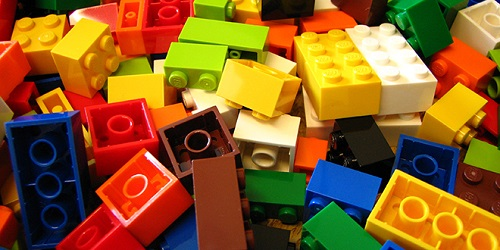
\includegraphics[width=.8\linewidth]{lego0}
\end{figure}
\end{frame}


\begin{frame}
	\begin{figure}
		\centering
		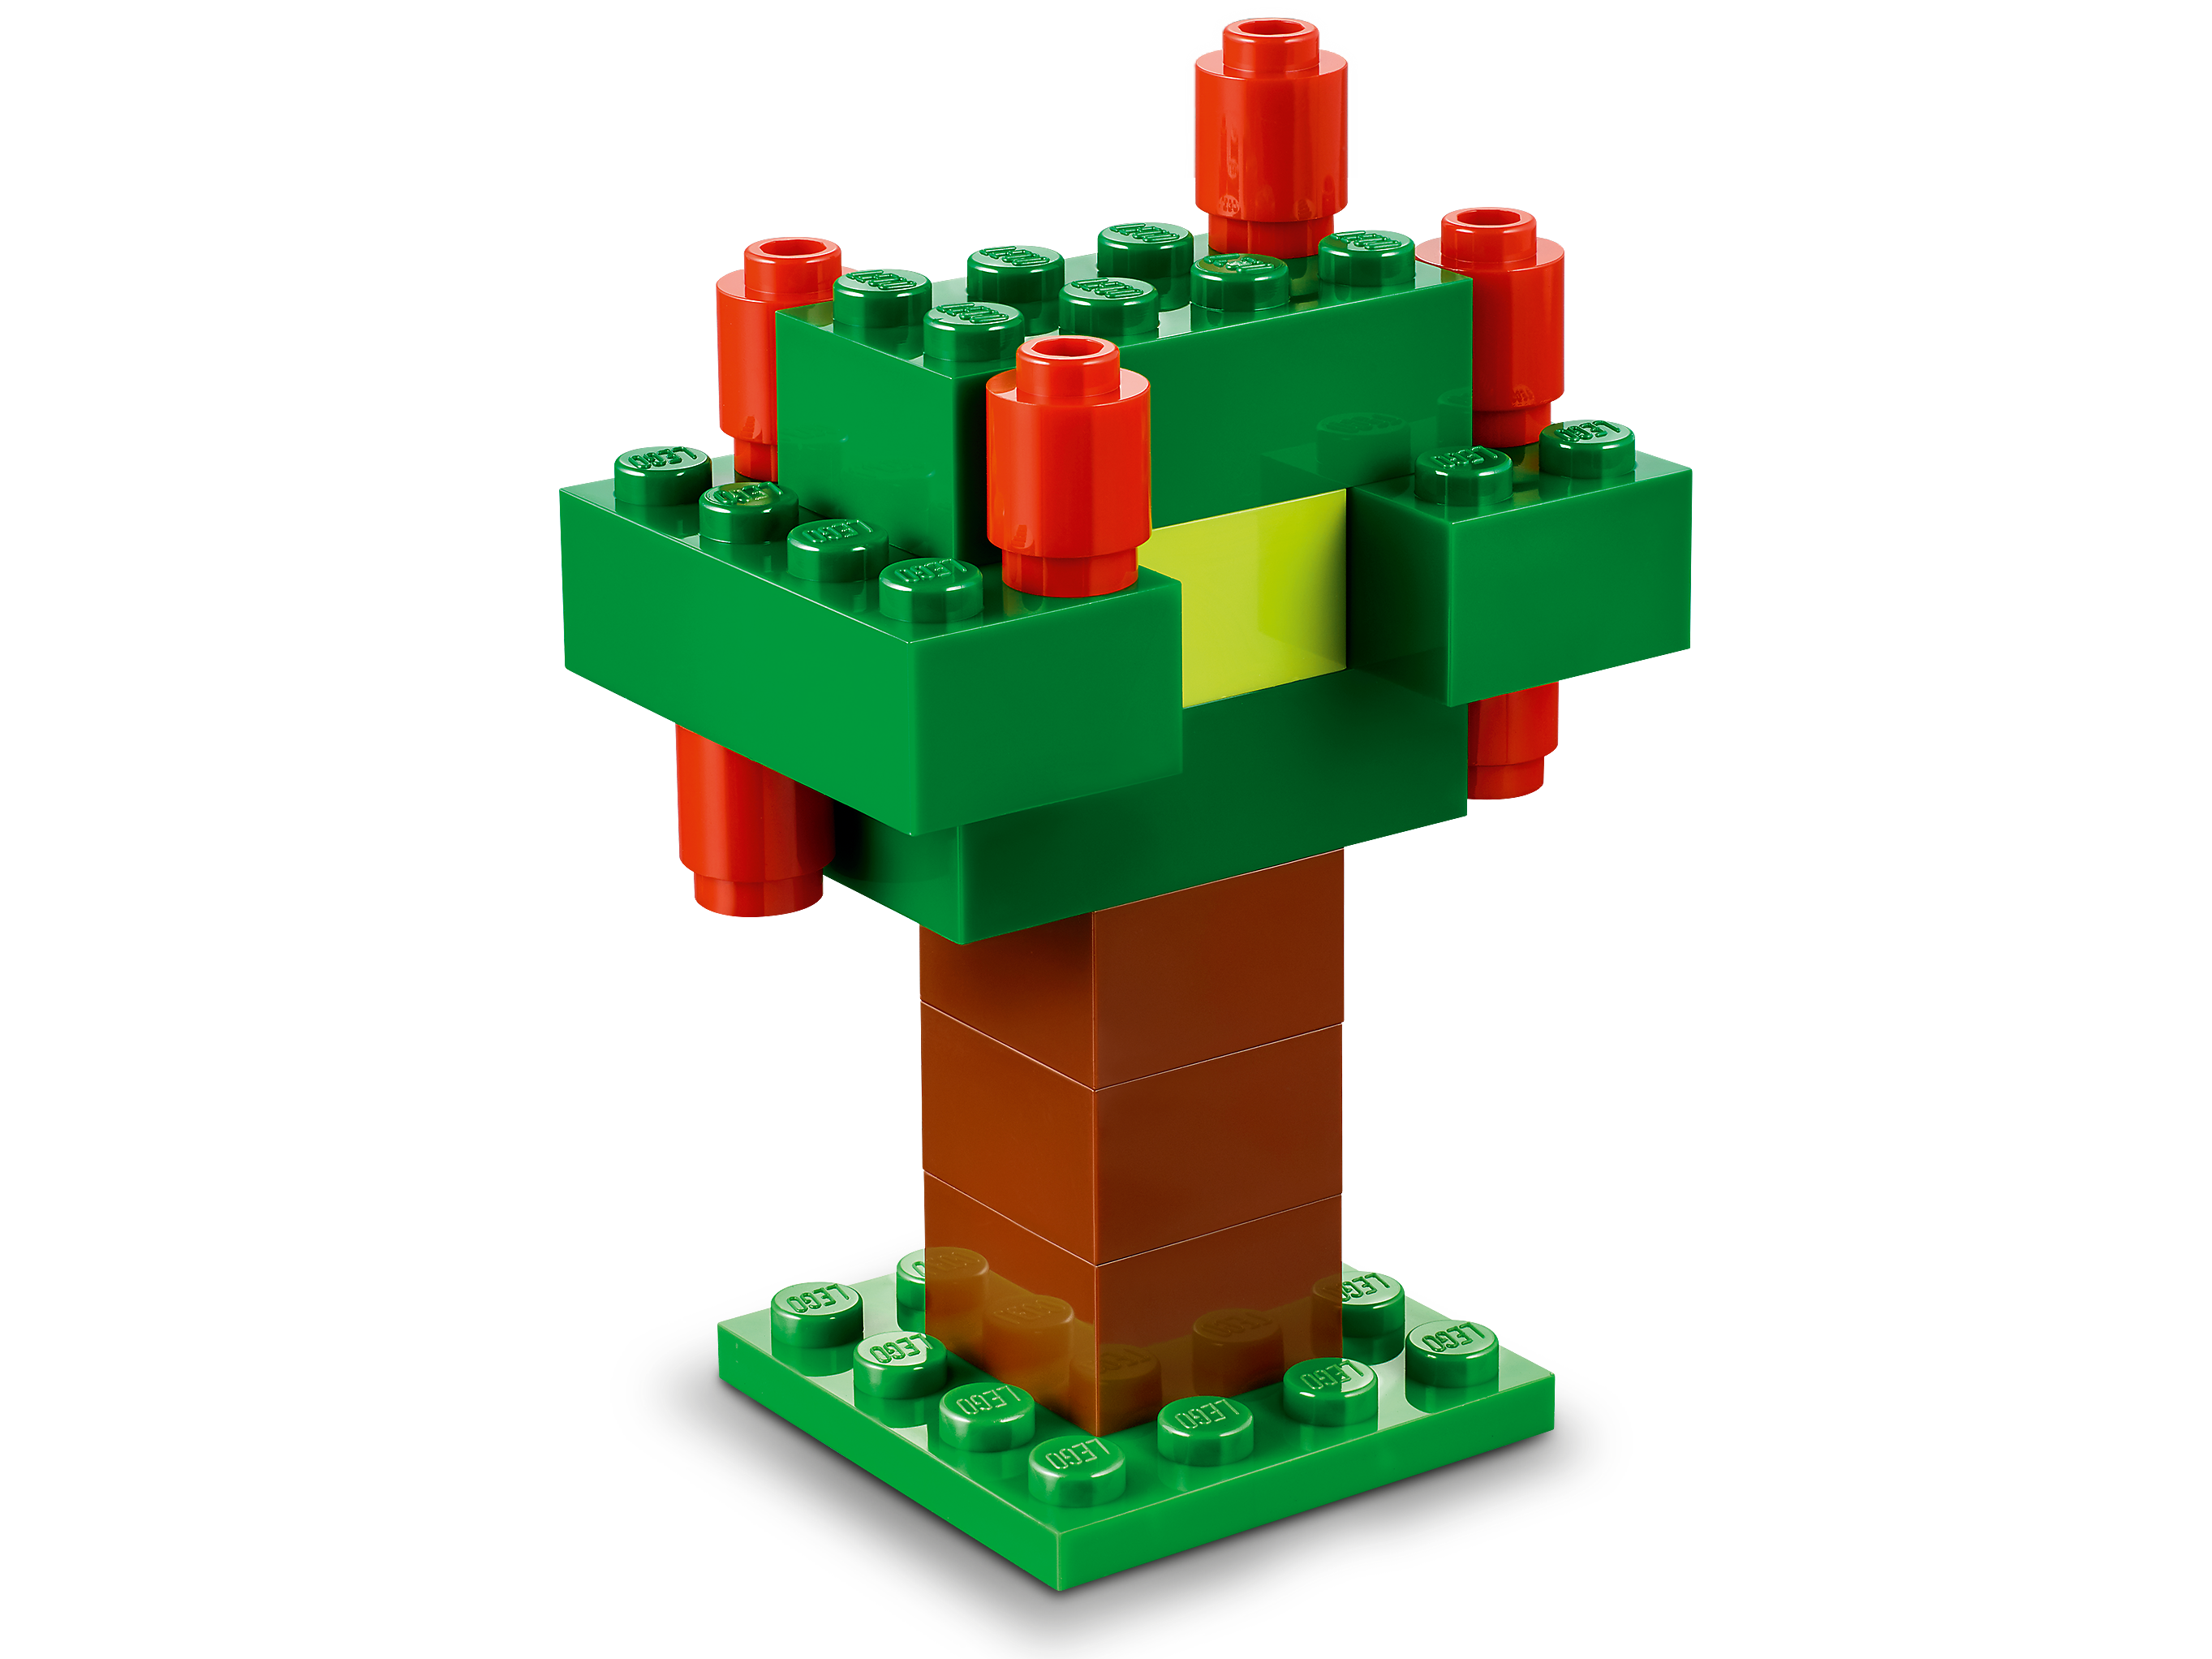
\includegraphics[width=.8\linewidth]{lego1}
	\end{figure}
\onslide<2->{The bricks, i.e. the individual elements build a model, representative of a reality.}
\end{frame}


\begin{frame}
\begin{itemize}
	
	\item In the \textbf{data analysis}, these bricks are the data
	\item Data that must be treated according to a given pattern - our statistical model - to recreate/represent an observed reality that we want to approximate.
\end{itemize}

\textbf{Why....?}
 to understand an explicit or hidden pattern inherent in the data  ... \textbf{why try to understand a pattern?}
	
\end{frame}

\begin{frame}
\small
\textbf{Interpret or predict}
\begin{itemize}
 \item To make decisions under conditions of uncertainty or even to anticipate upcoming scenarios and events.
 
 \item To this end, statistics uses probability to develop models with an underlying probabilistic nature to explain a given reality.
 
\end{itemize}

\begin{figure}
	\centering
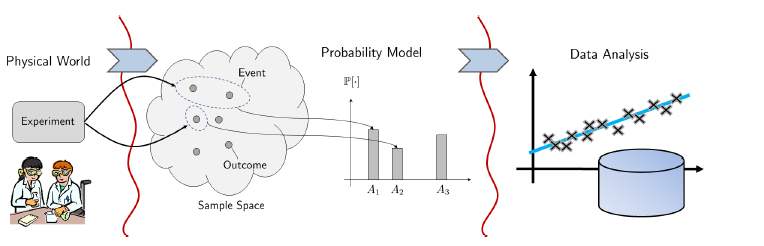
\includegraphics[width=.9\linewidth]{data_analisys}
\end{figure}

\textbf{but...}
\end{frame}

\begin{frame}
\begin{figure}
	
\end{figure}
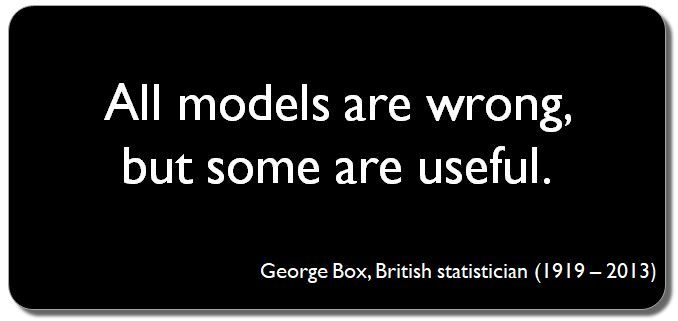
\includegraphics[width=.8\linewidth]{box}
We will \textbf{never} know the so-called data generating model, i.e. the real model designed by nature that has allowed the generation of data.

\end{frame}


%lego: cosa vediamo qui?
%sono dei lego, dei mattoncini che sostanzialmente assemblati in una certa maniera ci aiutano ad ottenere un risultato ... slide lego albero:

%possiamo dire che queti mattonci ci permettono di costruire un lemento unico piu grande che puo essere una rappresentazione piu o meno veritiera di qualcosa che esiste, quind i vediamo come il mattoncino cioè i singoli elmenti vanno a costruire un modello rappresentativo di una realta. una realta che esite e con noi andiamo ad approssimare. Nella analisi dati questi mattoncini possono essere intesi come i dati che vanno inseriti secondo un determinato schema che è il nostro modello statistico per ricreare una realtà che noi osserviamo e che vogliamo approssimare per capire uno schema insito nei dati esplicito o nascosto che estiste in questa realtà...perchè apire uno schema? per interpretare o predirre. Quinndi la comprensione ci permettera di prendere decisioni in condizioni di inertezza o addiritutra anticipare scenari od eventi prossimi non ancora verificati. A tal fine la statistica utilizza la probabilità per elaborare dei modelli con una natura sottostante probabilistica per spiegare una data realtà, tuttvia, il cdetto modello generatore dei dati, cioè il vero modello dettato dalla natura che ha permesso la generazione dei dati, non lo conosceremo mai.


%uno dei modelli piu semplici è quello lineare esempio classico è quello relazione consumi reddito, relazione cd lineare poichè puo essere rappresentata in maniera abbastanza precisa da una retta con una certa intercetta e un coeff angolare. Purtroppo pero la realtà non è sempre lineare, noi stimiamo una relazione ma la vera relazione che possono essere dati da fenomeni comportamentali fisici non la conosceremo mai ma la posiamo approssimare con un certo margine di errore, in questo caso la regressione lineare, che altro non è una retta stimata con un metodo probabilistico che va a stimare la migliore retta passante per certi punti 

\begin{frame}{Linear model}
	\begin{figure}
		\centering
		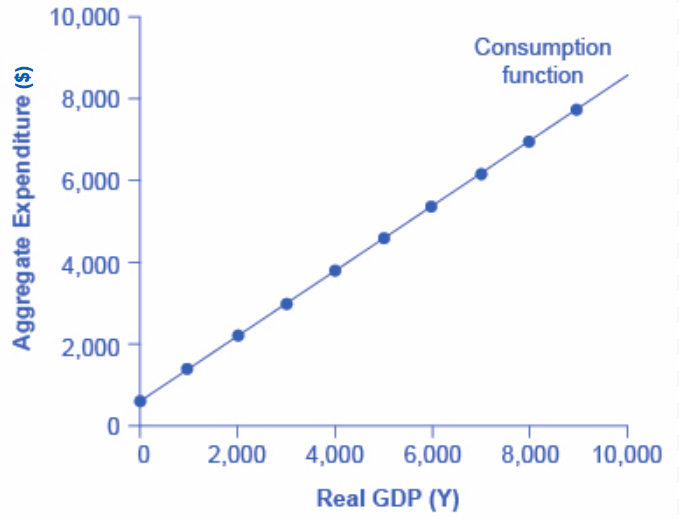
\includegraphics[width=.75\linewidth]{income}
	\end{figure}
\end{frame}

\section{What's deep learning}

\begin{frame}{Statistical learning is an evolution of statistical modeling}
	\footnotesize
	\centering
	\begin{figure}
		\centering
		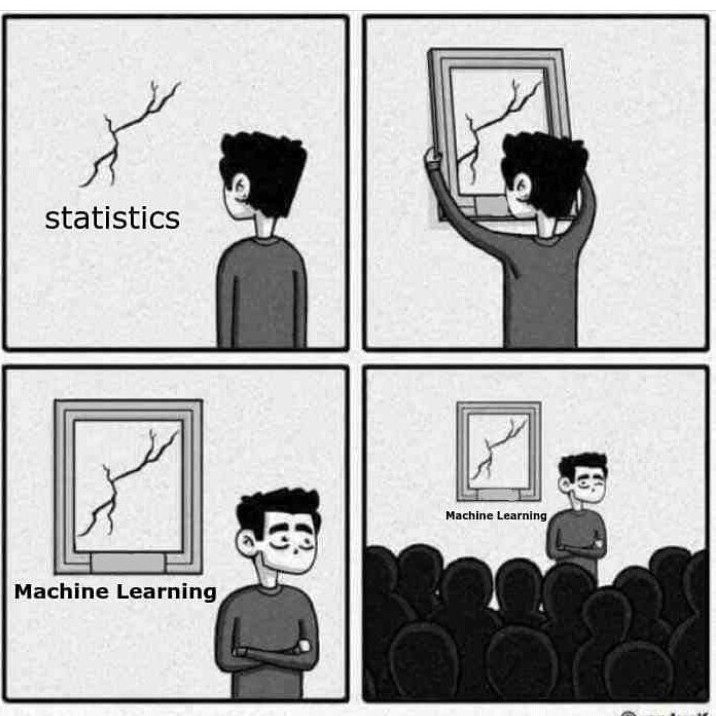
\includegraphics[width=.45\linewidth]{ML}

\begin{itemize}
				\tiny
	%\item Evolution of statistical modeling for predictioin purposes
		\item  for a given set of training data $\left\{\left(x_{1}, y_{1}\right) \ldots\left(x_{n}, y_{n}\right)\right\}$ sampled according to an unknown probability distribution $P(x, y)$, we find a function $f(\cdot)$ that minimises the expected error on a new test set of data:
			$$
			\int L(y, f(x)) P(x, y) d x d y
			$$
		\item	where $L(y, f(x))$ is the loss function that measures the prediction error for a given $x$ against the actual value $y$.			 
\end{itemize}
\end{figure}
\end{frame}

\begin{frame}{Statistics vs. Statistical Learning up to Machine Leaning}
	\footnotesize
	\centering
\textbf{Statistical Learning: New term...old concepts.}
	\begin{itemize}
		\item At the beginning of the nineteenth century - least squares 
		\item 1940s - logistic regression
		\item early 1970s, generalized linear model
	\end{itemize}
... they were almost linear methods because fitting non-linear relationships was computationally difficult. 

\end{frame}

\begin{frame}{Non-linear methods}
		\footnotesize
	\centering
	...By the 1980s, computing technology had finally improved sufficiently, that non-linear methods were no longer computationally prohibitive.
\begin{itemize}
	\item mid 1980s, regression trees and generalized additive models ... Neural networks gained popularity
	\item 1990 support vector machines
	\item Machine Learning: modern evolution of statistical learning
\end{itemize}
\end{frame}

\begin{frame}{Machine Leaning vs. Deep Learning}
		\small
\begin{itemize}
\item While all deep learning is machine learning, not all machine learning is deep learning
\item Machine Learning help the computer learn how to recognize things. This training requires a significant amount of human effort.
\item Deep learning algorithms: hierarchical models (multi-layered neural network) that does not require preprocessing.
\end{itemize}
\end{frame}


\begin{frame}{Time line}
\begin{figure}
	\centering
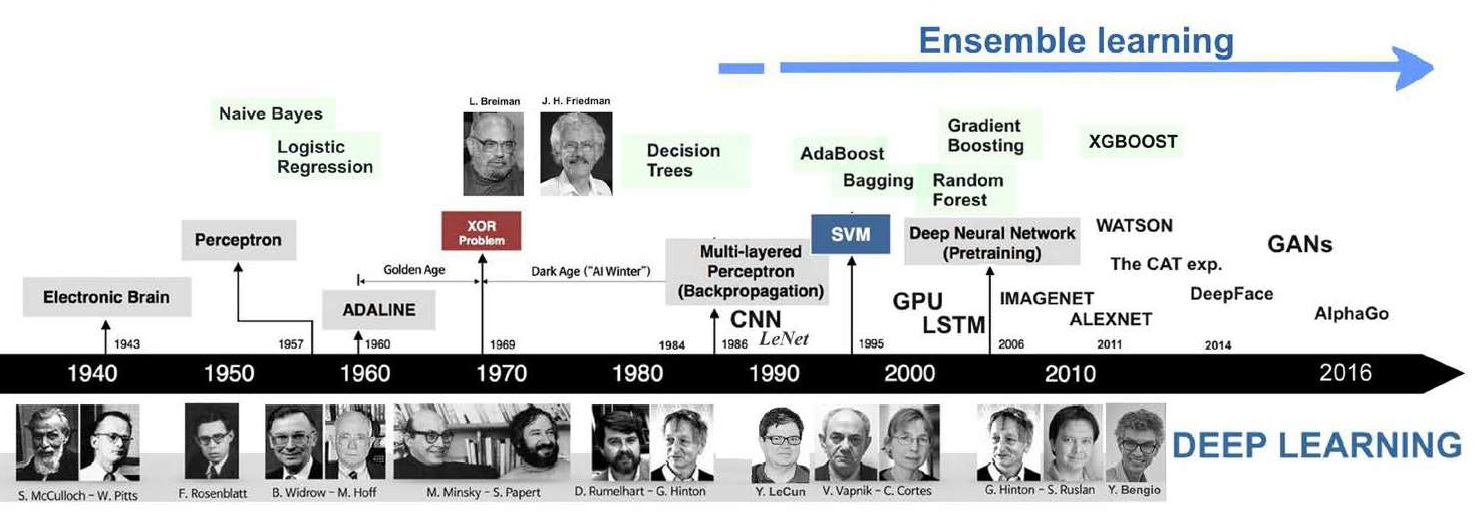
\includegraphics[width=1\linewidth]{story}		
\end{figure}
\end{frame}

\begin{frame}{Deep Learning: Deep Neural network}
	\small
\begin{figure}
	\centering
	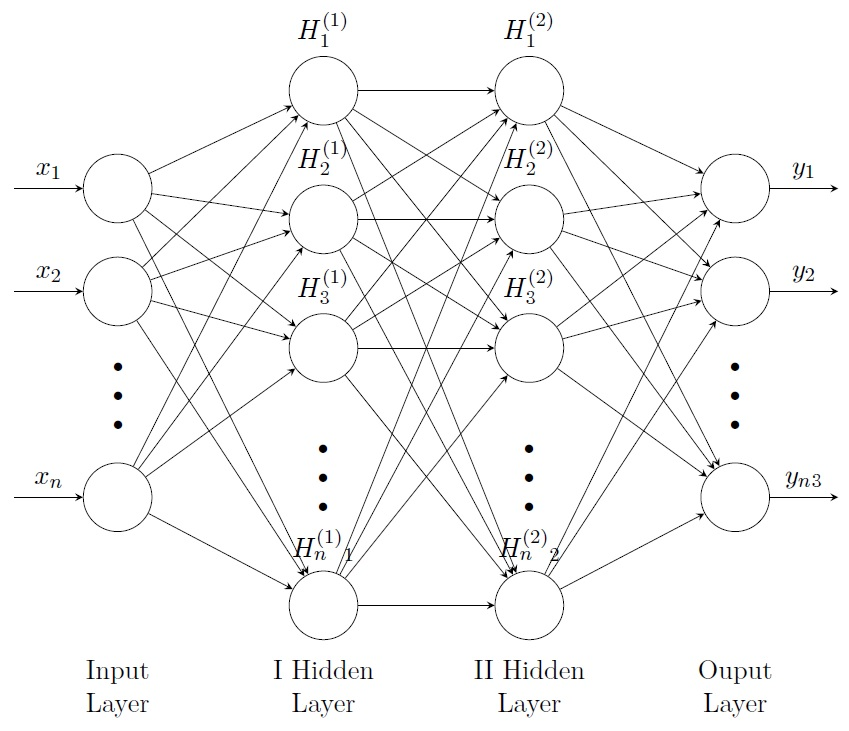
\includegraphics[width=.75\linewidth]{NNmodel}
\end{figure}
\end{frame}


\begin{frame}
\scriptsize
NN training involves an unconstrained optimization problem where the aim is to minimize a
function in high dimensional space the so-called loss function, that measures the difference between the predicted values and observed ones.
The back-propagation is the most used algorithm for the training of NNs. The algorithm compares the predicted values against the desired ones (objective)
and modifies the synaptic weights by back-propagating the gradient of the loss function. Schematically,
the procedure alternates forward and backward propagation steps:
\begin{itemize}
	\item in the forward step, the prediction is computed fixing the synaptic weights,
	\item in the backward step, the weights are adjusted in order to reduce the error of the network.
\end{itemize}

\end{frame}

\begin{frame}
	\scriptsize
The NN iteratively performs forward and backward propagation and modifies the weights to find the combination that minimizes the loss function	$$\mathcal{L}(y,\hat{y})=-\sum_{i=1}^{n} y_{i} \log \hat{y}_{i}+\left(1-y_{i}\right) \log \left(1-\hat{y}_{i}\right)$$

To minimize the loss function, we use the Gradient Descent optimization algorithm, that proceeds by minimizing $\mathcal{L}$ differentiating the loss function with respect to the weights  ($\mathbf{{W}}$).

The algorithm proceeds using the chain derivation rule described in the following equation:
\begin{equation}
	\frac{\partial \mathcal{L}(y,\hat{y})}{\partial w_{n,n}^{(k)}} =\frac{\partial \mathcal{L}(y,\hat{y})}{\partial H_n^{(k)}}\,\frac{{\partial H_n^{(k)}}}{\partial z_n^{(k)}} \, \frac{\partial z_n^{(k)}}{\partial w_{n,n}^{(k)}}
\end{equation}
where $ z_n^{(k)}=w_{n}^{(k)}\,H_{n}^{(k-1)}+b_n^{(k)}$. 
To update the weights ($\mathbf{\tilde{W}}$), the gradient of the loss function, $\nabla \mathcal{L}_t(y,\hat{y})$, is multiplied by a scalar, $\eta$, often called learning rate, according to the following scheme:
	\begin{equation}
	\mathbf{\tilde{W}}=\mathbf{W}-\eta \nabla \mathcal{L}_t(y,\hat{y})
\end{equation}
\end{frame}

\begin{frame}
	\scriptsize
	\begin{itemize}
	\item 	NN, like other machine learning techniques, requires the splitting of the dataset into a training and a testing set. The training set stands for supervised learning, while the testing set is used to
	validate the model. After the training phase, the network has learned the input–output functional relationship and it should be able to predict future values using only the input.
	\item The search for the optimal parameters is then carried out through an optimization process where the NN initial weights are selected in an arbitrary (random) way so they are not optimal parameters. The iterations of the algorithm lead to the optimization of the weights and minimization of the error. 
	The choices concerning the type of architecture (e.g., the number of hidden layers, units for each layer) and the hyperparameter (e.g., learning rate, activation functions, and loss function), remains a heuristic problem for NN users: the choice often depends on the type of data and it is not an easy step. 

	\end{itemize}
\end{frame}



\section{Case study}

\begin{frame}{Case Study}
\textit{Chinese consumers’ attitude towards ready to eat salads by comparing traditional Logit with Machine Learning methods}
\end{frame}

\begin{frame}
	\footnotesize
	\textbf{Motivation:}
	\begin{itemize}
	\item In the last decade, the ready to eat (RTE) food market has experienced substantial growth in China...but...
	\item ...No study offers an attitudinal and behavioral analysis of the topic
	\item A survey among Chinese respondents to understand the factors associated with RTE salad consumption
	\end{itemize}

	\textbf{Contribution:}
	\begin{itemize}
	\item \textbf{First,} we aim at profiling the typical consumer of RTE salads
	\item \textbf{Second,} we test different machine learning classification algorithms on primary consumer data.
	\end{itemize}


 \end{frame}


 \begin{frame}
 	\footnotesize
\textbf{Results 1: consumption is more common among}
\begin{itemize}
	\item young respondents,  
	\item females,
	\item healthy-oriented individuals at the beginning of their career,
	\item the role of the subjective norm (other people influence on our choices) is positively associated with increased consumption of RTE salads. 
\end{itemize}		

\textbf{Results 2: Best predictive models}
\begin{itemize}
	\item RT
	\item RF
	\item SVM
	\item DNN
\end{itemize}		 	
\end{frame}

%\begin{frame}
%	\tiny
%	\begin{table}[H]
%		\begin{tabular}{l|l|l|l}
%			\hline
%			\textbf{Variable}                 & \textbf{Frequency} & \textbf{Variable}                              &% \textbf{Frequency} \\ \hline
%			\textbf{Gender}                   & \textit{}          & \textbf{Regular consumption of RTE}            & \textit{}          \\ \hline
%			\textit{Female}                   & \textit{52\%}      & salads                                         & \textit{}          \\ \hline
%			\textit{Male}                     & \textit{48\%}      & \textit{Yes}                                   & \textit{25\%}      \\ \hline
%			\textbf{Age}                      & \textit{}          & \textit{No}                                    & \textit{75\%}      \\ \hline
%			\textit{21-25}                    & \textit{23\%}      & \textbf{Fitness}                               & \textit{}          \\ \hline
%			\textit{26-30}                    & \textit{34\%}      & \textit{Yes}                                   & \textit{48\%}      \\ \hline
%			\textit{31-35}                    & \textit{12\%}      & \textit{No}                                    & \textit{52\%}      \\ \hline
%			\textit{36-40}                    & \textit{17\%}      & \textbf{Learning-advertising}        &                    \\ \hline
%			\textit{\textgreater{}40}         & \textit{14\%}      & \textit{Yes}                                   & \textit{76\%}      \\ \hline
%			\textbf{Income}                   & \textit{}          & \textit{No}                                    & \textit{24\%}      \\ \hline
%			\textit{Below 15,000rmb}          & \textit{28\%}      & \textbf{Learning-social media}       &                    \\ \hline
%			\textit{Between 15 and 20,000rmb} & \textit{25\%}      & \textit{Yes}                                   & \textit{31\%}      \\ \hline
%			\textit{Between 20 and 25,000rmb} & \textit{21\%}      & \textit{No}                                    & \textit{69\%}      \\ \hline
%			\textit{More than 25,000rmb}      & \textit{27\%}      & \textbf{Purchasing-supermarket}       & \textit{}          \\ \hline
%			\textbf{Job seniority level}      & \textit{}          & \textit{Yes}                                   & \textit{75\%}      \\ \hline
%			\textit{Entry}                    & \textit{40\%}      & \textit{No}                                    & \textit{25\%}      \\ \hline
%			\textit{Middle}                   & \textit{45\%}      & \textbf{Purchasing-convenience store} & \textit{}          \\ \hline
%			\textit{Managerial}               & \textit{15\%}      & \textit{Yes}                                   & \textit{49\%}      \\ \hline
%			\textbf{Household size}           & \textit{}          & \textit{No}                                    & \textit{51\%}      \\ \hline
%			\textit{One or two people}        & \textit{18\%}      & \textbf{Consumption for snacking}              & \textit{}          \\ \hline
%			\textit{Three people}             & \textit{50\%}      & \textit{Yes}                                   & \textit{60\%}      \\ \hline
%			\textit{More than three people}   & \textit{32\%}      & \textit{No}                                    & \textit{40\%}      \\ \hline
%			\textbf{Knowledge of RTE}         & \textit{}          & \textbf{Consumption for lunch}                 & \textit{}          \\ \hline
%			\textit{Low}                      & \textit{25\%}      & \textit{Yes}                                   & \textit{60\%}      \\ \hline
%			\textit{Medium}                   & \textit{39\%}      & \textit{No}                                    & \textit{40\%}      \\ \hline
%			\textit{High}                     & \textit{36\%}      &                                                & \textit{}          \\ \hline
%			
		%	\textbf{Subjective norm}          & \textit{}          & \textbf{}                 & \textit{}          %\\ \hline
	%		\textit{Low}                      & \textit{10.79\%}      & \textit{}                                   & \textit{60\%}      \\ \hline
%			\textit{Medium}                   & \textit{51.76\%}      & \textit{}                                    & \textit{40\%}      \\ \hline
%			\textit{High}                     & \textit{37.44\%}      &                                                & \textit{}          \\ \hline
			
%		\end{tabular}
%		\caption{Descriptive Statistics}
%		\label{table:statistics}
%	\end{table}
%\end{frame}


\begin{frame}{Data}
	\scriptsize
	\begin{table}[H]
		\begin{tabular}{l|l|l|l}
			\hline
			\textbf{Variable}                 & \textbf{Frequency} & \textbf{Variable}                              & \textbf{Frequency} \\ \hline
			\textbf{Gender}                   & \textit{}          & \textbf{Regular consumption of RTE}            & \textit{}          \\ \hline
			\textit{Female}                   & \textit{52\%}      & salads                                         & \textit{}          \\ \hline
			\textit{Male}                     & \textit{48\%}      & \textit{Yes}                                   & \textit{25\%}      \\ \hline
			\textbf{Age}                      & \textit{}          & \textit{No}                                    & \textit{75\%}      \\ \hline
			\textit{21-25}                    & \textit{23\%}      & \textbf{Fitness}                               & \textit{}          \\ \hline
			\textit{26-30}                    & \textit{34\%}      & \textit{Yes}                                   & \textit{48\%}      \\ \hline
			\textit{31-35}                    & \textit{12\%}      & \textit{No}                                    & \textit{52\%}      \\ \hline
			\textit{36-40}                    & \textit{17\%}      & \textbf{Learning-advertising}        &                    \\ \hline
			\textit{\textgreater{}40}         & \textit{14\%}      & \textit{Yes}                                   & \textit{76\%}      \\ \hline
			\textbf{Income}                   & \textit{}          & \textit{No}                                    & \textit{24\%}      \\ \hline
			\textit{Below 15,000rmb}          & \textit{28\%}      & \textbf{Learning-social media}       &                    \\ \hline
			\textit{Between 15 and 20,000rmb} & \textit{25\%}      & \textit{Yes}                                   & \textit{31\%}      \\ \hline
			\textit{Between 20 and 25,000rmb} & \textit{21\%}      & \textit{No}                                    & \textit{69\%}      \\ \hline
			\textit{More than 25,000rmb}      & \textit{27\%}      & \textbf{}       & \textit{}          \\ \hline
					
		\end{tabular}
		\caption{Descriptive Statistics}
		\label{table:statistics}
	\end{table}
\end{frame}

\begin{frame}{Data}
	\scriptsize
	\begin{table}[H]
		\begin{tabular}{l|l|l|l}
			\hline
			\textbf{Variable}                 & \textbf{Frequency} & \textbf{Variable}                              & \textbf{Frequency} \\ \hline
			 & & \textbf{Purchasing-supermarket}       & \textit{}          \\ \hline
			\textbf{Job seniority level}      & \textit{}          & \textit{Yes}                                   & \textit{75\%}      \\ \hline
			\textit{Entry}                    & \textit{40\%}      & \textit{No}                                    & \textit{25\%}      \\ \hline
			\textit{Middle}                   & \textit{45\%}      & \textbf{Purchasing-convenience store} & \textit{}          \\ \hline
			\textit{Managerial}               & \textit{15\%}      & \textit{Yes}                                   & \textit{49\%}      \\ \hline
			\textbf{Household size}           & \textit{}          & \textit{No}                                    & \textit{51\%}      \\ \hline
			\textit{One or two people}        & \textit{18\%}      & \textbf{Consumption for snacking}              & \textit{}          \\ \hline
			\textit{Three people}             & \textit{50\%}      & \textit{Yes}                                   & \textit{60\%}      \\ \hline
			\textit{More than three people}   & \textit{32\%}      & \textit{No}                                    & \textit{40\%}      \\ \hline
			\textbf{Knowledge of RTE}         & \textit{}          & \textbf{Consumption for lunch}                 & \textit{}          \\ \hline
			\textit{Low}                      & \textit{25\%}      & \textit{Yes}                                   & \textit{60\%}      \\ \hline
			\textit{Medium}                   & \textit{39\%}      & \textit{No}                                    & \textit{40\%}      \\ \hline
			\textit{High}                     & \textit{36\%}      &                                                & \textit{}          \\ \hline
			
			\textbf{Subjective norm}          & \textit{}          & \textbf{}                 & \textit{}          \\ \hline
			\textit{Low}                      & \textit{10.79\%}      & \textit{}                                   & \textit{}      \\ \hline
			\textit{Medium}                   & \textit{51.76\%}      & \textit{}                                    & \textit{}      \\ \hline
			\textit{High}                     & \textit{37.44\%}      &                                                & \textit{}          \\ \hline
			
		\end{tabular}
		
		\label{table:statistics}
	\end{table}
\end{frame}
















\begin{frame}{Accuracy prediction}
	\scriptsize
\begin{table}[]
	\begin{tabular}{|l|l|l|}
		\hline
		$\hat{y}/y$ & 1                         & 0                         \\ \hline
		1           & TP                        & FP                        \\ \hline
		0           & FN                        & TN                        \\ \hline
		& Sens: $\frac{TP}{TP+FN}$ & Spec: $\frac{TN}{TN+FP}$ \\ \hline
	\end{tabular}
\end{table}
	
For binary target variables, we evaluate the level of accuracy, true positive rate (Sensitivity) and true negative rate (Specificity). We define  $y=1$ for a regular consuption of RTE and 0 otherwise. Then a $2 \times 2$ confusion matrix has elements $a_{\text {row,column }}$ with predicted conditions $\widehat{y}=\{1,0\}$ on rows and true conditions $y=\{1,0\}$ on columns. The statistics are defined by: $\text{Accuracy }=\frac{TP+TN}{TP+FP+FN+TN}$

\end{frame}

\begin{frame}{Accuracy prediction}
	\scriptsize
\begin{itemize}
	\item We calculate accuracy that refers to the portion of customers correctly classified with respect to RTE regular consumption.
	
	\item Sensitivity (true positive rate) refers to the proportion of regular RTE consumers correctly identified as such. Poor sensitivity implies a large number of inclusion errors, i.e. identifying RTE consumers when in fact they are not.
	\item   Specificity (true negative rate) refers to the proportion of customers correctly predicted to be occasional RTE consumers. Poor specificity implies a large number of exclusion errors. 
\end{itemize}


The reported output will provide the numerical and graphical representation of the ROC curve and the relative area under the curve (AUC) values. The area under the (ROC) curve, summarizes the classifier performance. The larger area under the curve the better the classifier.
\end{frame}

\begin{frame}{Accuracy prediction}
		\small
	\begin{figure}
		\centering
		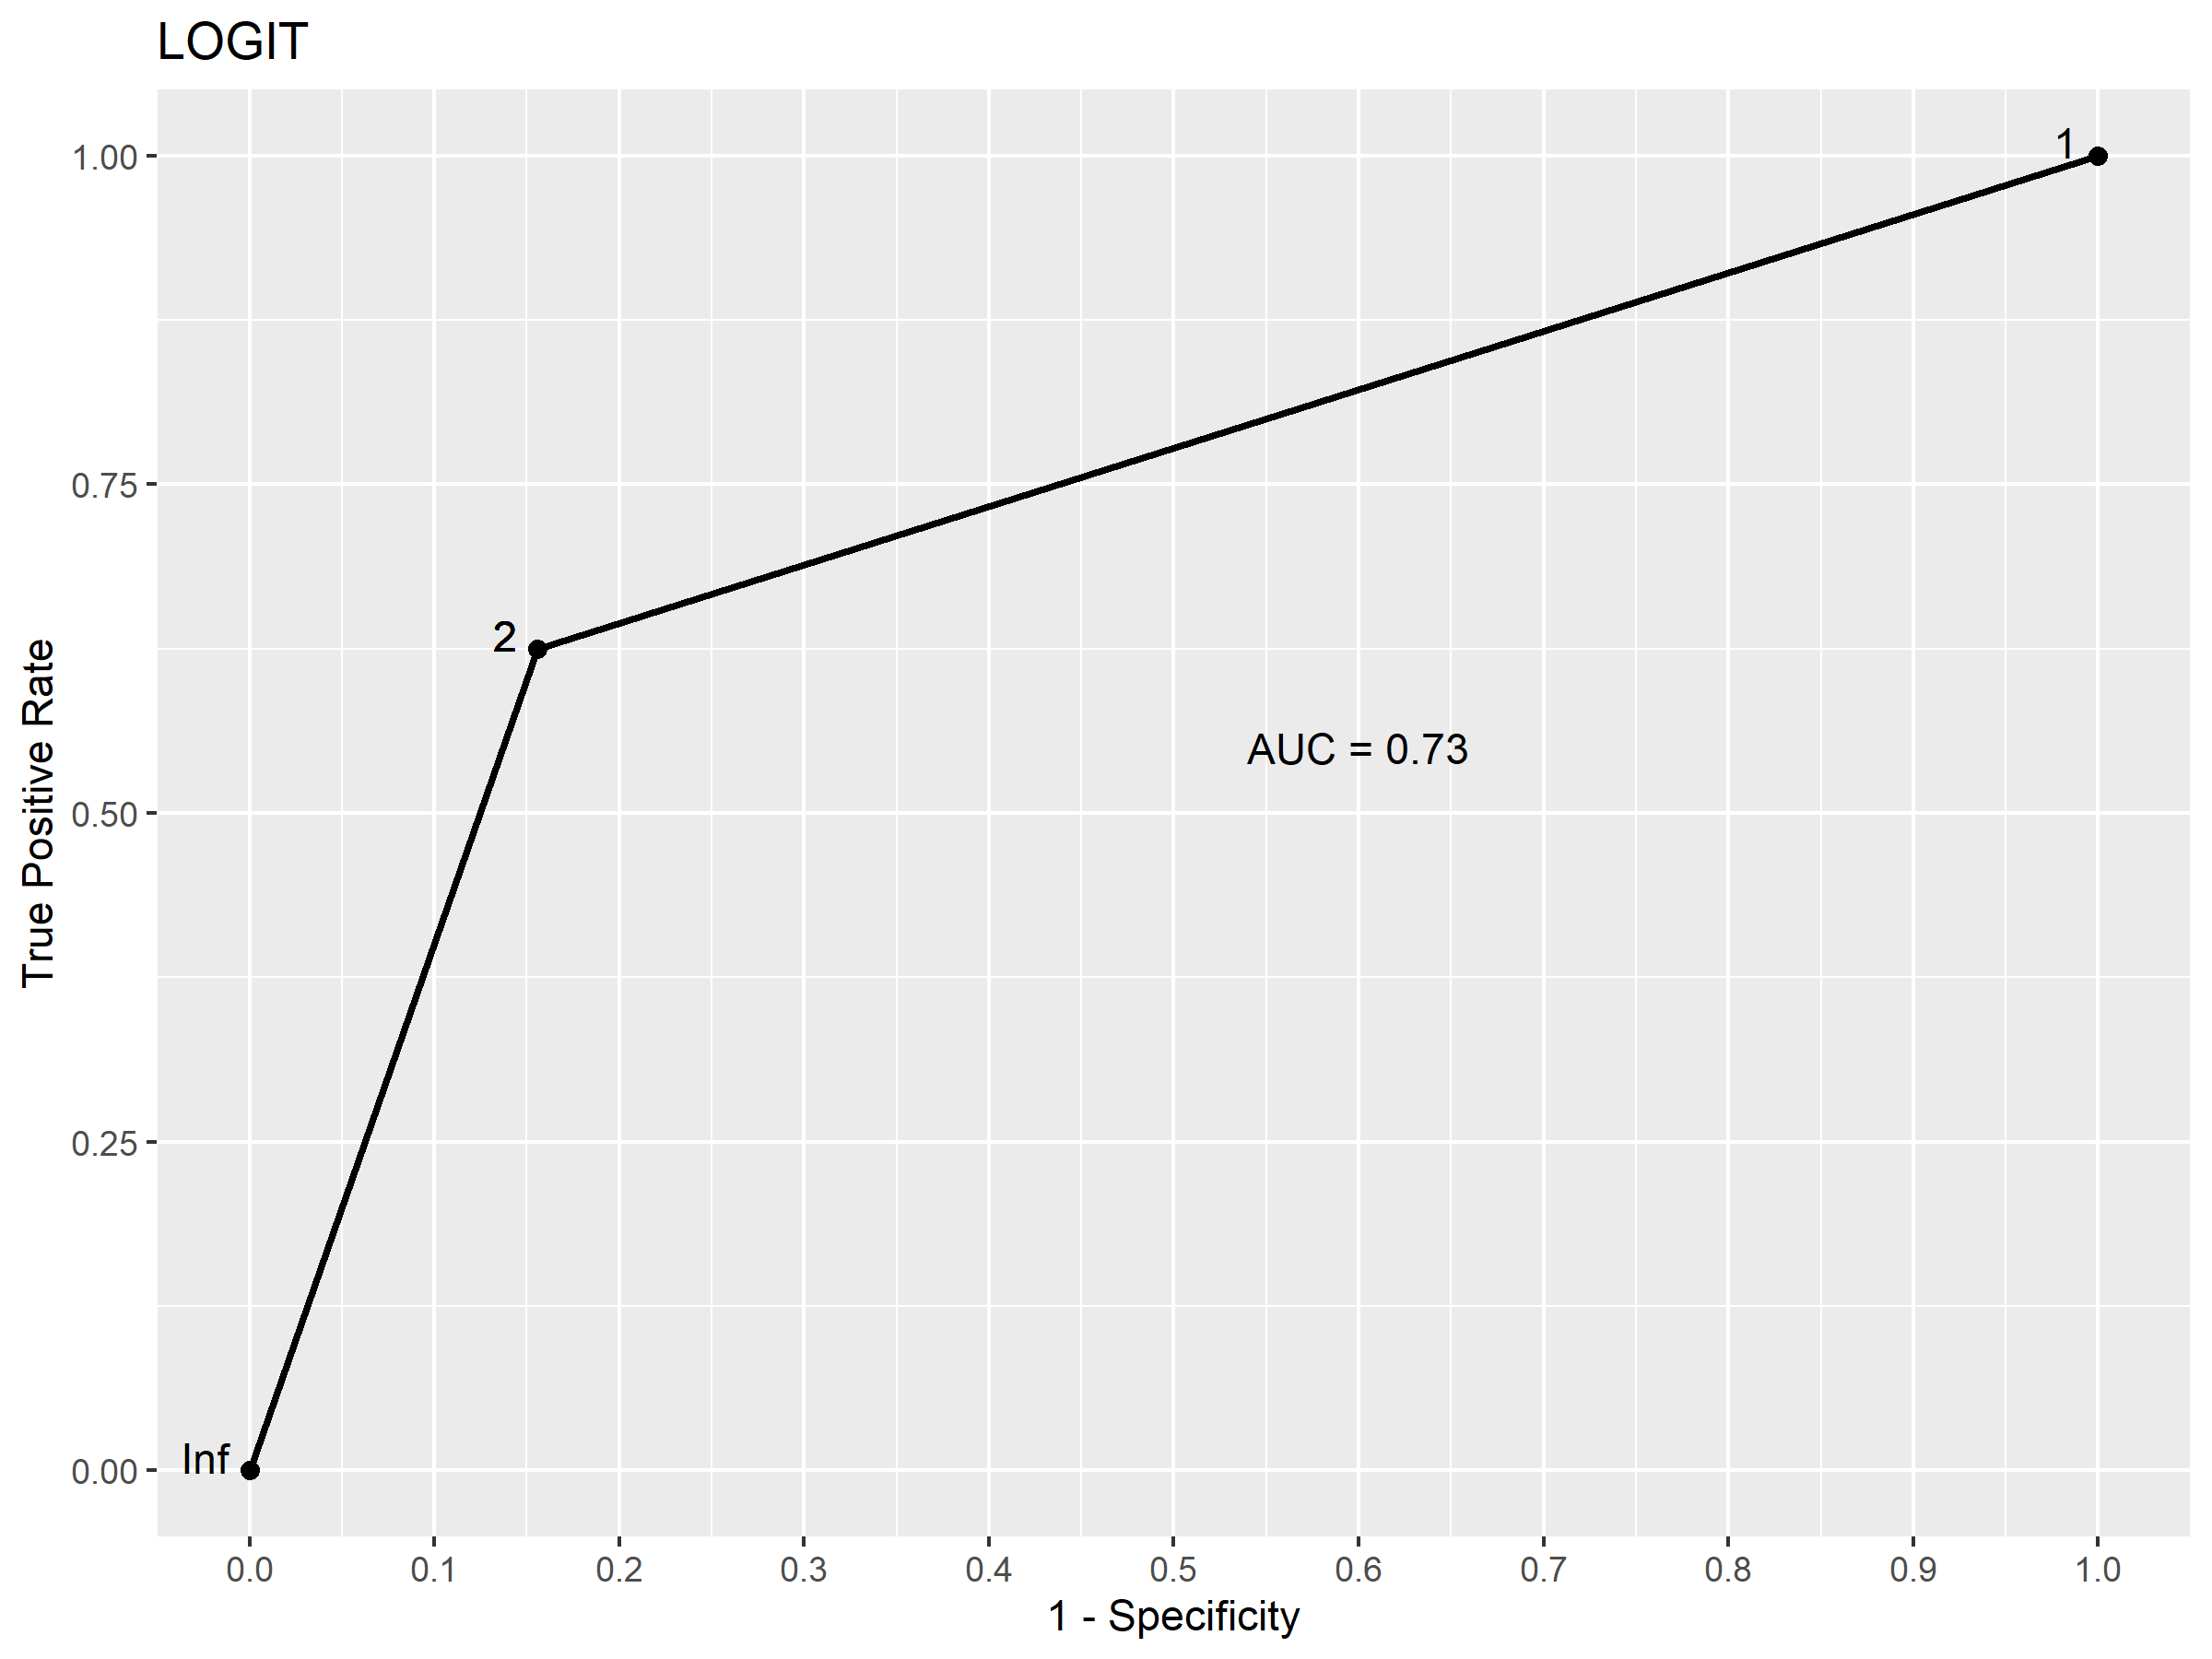
\includegraphics[width=.8\linewidth]{logit}
	\end{figure}
\end{frame}

\section{Let's go to practice.}


%\begin{frame}
%	\Huge \textbf{Thank you for your attention.}\\
%	\bigskip
%\end{frame}

%\begin{frame}{References}
%\end{frame}

\end{document}